% !Mode:: "TeX:UTF-8"
% !TEX encoding = UTF-8 Unicode

%----------------------------------------------------------------------------------------
% 机器翻译:基础与模型
% Machine Translation: Foundations and Models
%
% Copyright 2020
% 肖桐(xiaotong@mail.neu.edu.cn) 朱靖波 (zhujingbo@mail.neu.edu.cn)
%----------------------------------------------------------------------------------------

%----------------------------------------------------------------------------------------
%    CONFIGURATIONS
%----------------------------------------------------------------------------------------

\renewcommand\figurename{图}%将figure改为图
\renewcommand\tablename{表}%将figure改为图
\chapterimage{fig-NEU-8.jpg} % Chapter heading image

%----------------------------------------------------------------------------------------
%	CHAPTER 18
%----------------------------------------------------------------------------------------

\chapter{机器翻译应用技术}

\parinterval 随着机器翻译品质的不断提升,越来越多的应用需求被挖掘出来。但是,一个优秀的机器翻译引擎并不意味着机器翻译可以被成功应用。机器翻译技术落地需要“额外”考虑很多因素,例如,数据处理方式、交互方式、应用的领域等,甚至机器翻译模型也要经过改造才能适应到不同的场景中。

\parinterval 本章将重点介绍机器翻译应用中所面临的一些实际问题,以及解决这些问题可以采用的策略。本章所涉及的内容较为广泛,一方面会大量使用本书前十七章的模型和方法,另一方面也会介绍新的技术手段。最终,本章会结合机器翻译的特点展示一些机器翻译可以应用的场景。

%----------------------------------------------------------------------------------------
%    NEW SECTION
%----------------------------------------------------------------------------------------

\section{机器翻译的应用并不简单}

\parinterval 近几年,无论从评测比赛的结果,还是论文发表数量上看,机器翻译的研究可谓火热。但是,客观的说,我们离机器翻译完美的应用还有相当的距离。这主要是因为,成熟的系统需要很多技术的融合。因此,机器翻译系统研发也是一项复杂的系统工程。而机器翻译研究大多是对局部模型和方法的调整,这也会造成一个现象:很多论文里报道的技术方法可能无法直接应用于真实场景的系统。这里,有几方面挑战:

\begin{itemize}
\vspace{0.5em}
\item 机器翻译模型很脆弱。实验环境下,给定翻译任务,甚至给定训练和测试数据,机器翻译模型可以表现得很好。但是,应用场景是不断变化的。经常会出现训练数据缺乏、应用领域与训练数据不匹配、用户的测试方法与开发者不同等等一系列问题。特别是,对于不同的任务,神经机器翻译模型需要进行非常细致的调整,理想中“一套包打天下”的模型和设置是不存在的。这些都导致一个结果:直接使用既有机器翻译模型很难满足不断变化的应用需求。

\vspace{0.5em}
\item 机器翻译缺少针对场景的应用技术。目前为止,机器翻译的研究进展已经为我们提供很好的机器翻译基础模型。但是,用户并不是简单的与这些模型“打交道”,他们更加关注如何解决自身的业务需求,例如,机器翻译应用的交互方式、系统是否可以自己预估翻译可信度等等。甚至,在某些场景中,用户对翻译模型占用的存储空间和运行速度都有非常严格的要求。

\vspace{0.5em}
\item 优秀系统的研发需要长时间的打磨。工程打磨也是研发优秀机器翻译系统的必备条件,有些时候甚至是决定性的。从科学研究的角度看,我们需要对更本质的科学问题进行探索,而非简单的工程开发与调试。但是,对一个初级的系统进行研究往往会掩盖掉“真正的问题”,因为很多问题在更优秀的系统中并不存在。
\vspace{0.5em}
\end{itemize}

\parinterval 下面本章将重点对机器翻译应用中的若干技术问题展开讨论,旨在给机器翻译应用提供一些可落地的思路。

%----------------------------------------------------------------------------------------
%    NEW SECTION
%----------------------------------------------------------------------------------------

\section{增量式模型优化}

\parinterval 机器翻译的训练数据不是一成不变的。系统研发人员可以使用自有数据训练得到基础的翻译模型(或初始模型)。当应用这个基础模型时,可能会有新的数据出现,例如:

\begin{itemize}
\vspace{0.5em}
\item 应用的目标领域和场景可能是研发系统时无法预见的,但是用户会有一定量的自有数据,可以用于系统优化。
\vspace{0.5em}
\item 系统在应用中会产生新的数据,这些数据经过一些筛选和修改也可以用于模型训练。
\vspace{0.5em}
\end{itemize}

\parinterval 这时就产生一个问题,能否使用新的数据让系统变得更好?简单直接的方式是,将新的数据和原始数据混合重新训练系统,但是使用全量数据训练模型的周期很长,这种方法的成本很高。而且,新的数据可能是不断产生的,甚至是流式的。这时就需要一种快速、低成本的方式对模型进行更新。

\parinterval 增量训练就是满足上述需求的一种方法。{\chapterthirteen}已经就增量训练这个概念展开了一些讨论,这里重点介绍一些具体的实践手段。本质上,神经机器翻译中使用的随机梯度下降方法就是典型的增量训练方法,其基本思想是:每次选择一个样本对模型进行更新,这个过程反复不断执行,每次模型更新都是一次增量训练。当多个样本构成了一个新数据集时,可以把这些新样本作为训练数据,把当前的模型作为初始模型,之后正常执行机器翻译的训练过程即可。如果新增加的数据量不大(比如,几万句对),训练的代价非常低。

\parinterval 这里面的一个问题是,新的数据虽然能代表一部分的翻译现象,但是如果仅仅依赖新数据进行更新,会使模型对新数据过分拟合,从而无法很好地处理新数据之外的样本。这也可以被看做是一种灾难性遗忘的问题\upcite{DBLP:conf/coling/GuF20},即:模型过分注重对新样本的拟合,丧失了旧模型的一部分能力。在实际系统开发中,有几种常用的增量训练方法:

\begin{itemize}
\vspace{0.5em}
\item 数据混合\upcite{DBLP:journals/corr/ChuDK17}。在增量训练时,除了使用新的数据,再混合一定量的旧数据,混合的比例可以根据训练的代价进行调整。这样,模型相当于在全量数据的一个采样结果上进行更新。

\vspace{0.5em}
\item 模型插值\upcite{DBLP:conf/emnlp/WangULCS17}。在增量训练之后,将新模型与旧模型进行插值。

\vspace{0.5em}
\item 多目标训练\upcite{barone2017regularization,DBLP:conf/aclnmt/KhayrallahTDK18,DBLP:conf/naacl/ThompsonGKDK19}。在增量训练时,除了在新数据上定义损失函数之外,可以再定义一个在旧数据上的损失函数,这样确保模型可以在两个数据上都有较好的表现。也可以在损失函数中引入正则化项,使新模型的参数不会偏离旧模型的参数太远。

\vspace{0.5em}
\end{itemize}

\parinterval 图\ref{fig:18-1}给出了上述方法的对比。在实际应用中,还有很多细节会影响增量训练的效果,比如,学习率大小的选择等。另外,新的数据积累到何种规模可以进行增量训练也是实践中需要解决的问题。一般来说,增量训练使用的数据量越大,训练的效果越稳定。但是,这并不是说数据量少就不可以进行增量训练,而是如果数据量过少时,需要考虑训练代价和效果之间的平衡。而且,过于频繁的增量训练也会带来更多的灾难性遗忘的风险,因此合理进行增量训练也是机器翻译应用中需要实践的。

%----------------------------------------------
\begin{figure}[htp]
\centering
\addtolength{\tabcolsep}{-4pt}

\begin{tabular}{c c c}

\begin{tikzpicture}
\begin{scope}
% ,minimum height =1em,minimum width=2em
\tikzstyle{model} = [draw,black,very thick,inner sep=3.5pt,rounded corners=4pt,fill=blue!20,minimum width=4em,minimum height=1.5em,font=\footnotesize]
\tikzstyle{data} = [draw,black,very thick,inner sep=3.5pt,rounded corners=4pt,fill=green!20,minimum width=4em,minimum height=1.5em,font=\footnotesize]
\tikzstyle{data2} = [draw,black,very thick,inner sep=3.5pt,rounded corners=4pt,minimum width=2em,minimum height=1.5em,font=\footnotesize]

\tikzstyle{word} = [inner sep=3.5pt,font=\footnotesize]

\node[data2,fill=green!60] (old) at (0,0) {};
\node[data2,fill=green!20] (old2) at ([xshift=0.9em]old.east) {};
\node[word] at (0.1,0.5) {旧数据};

\node[data] (new) at ([xshift=3em]old2.east) {新数据};
\node[data] (all) at ([xshift=2.55em,yshift=-4em]old.south) {最终数据};
\node[model] (final_model) at ([xshift=0em,yshift=-4em]all.south) {最终模型};

\draw [->,thick] ([yshift=-0.2em]old2.south) .. controls +(south:2.5em) and +(north:2.5em) .. ([xshift=-0.2em,yshift=0.2em]all.north);
\draw [->,thick] ([yshift=-0.2em]new.south) .. controls +(south:2.5em) and +(north:2.5em) .. ([xshift=0.2em,yshift=0.2em]all.north);
\draw [->,thick] ([yshift=-0.2em]all.south) -- ([yshift=0.2em]final_model.north)node[pos=0.5,right,align=center,font=\footnotesize] {训练};

\node[word] at ([yshift=-2em]final_model.south){(a)数据混合};

\begin{pgfonlayer}{background}
\node [rectangle,inner sep=0.5em,rounded corners=1pt,minimum width=4.5em,minimum height=3.2em,draw=red!50,dotted,very thick] at (0.37,0.15) {};

\end{pgfonlayer}

\end{scope}
\end{tikzpicture}
&
\begin{tikzpicture}
\begin{scope}
\tikzstyle{model} = [draw,black,very thick,inner sep=3.5pt,rounded corners=4pt,fill=blue!20,minimum width=4em,minimum height=1.5em,font=\footnotesize]
\tikzstyle{data} = [draw,black,very thick,inner sep=3.5pt,rounded corners=4pt,fill=green!20,minimum width=4em,minimum height=1.5em,font=\footnotesize]
\tikzstyle{word} = [inner sep=3.5pt,font=\footnotesize]

\node[data] (old) at (0,0) {旧数据};
\node[data] (new) at ([xshift=3em]old.east) {新数据};
\node[model] (old_model) at ([yshift=-4em]old.south) {旧模型};
\node[model] (new_model) at ([yshift=-4em]new.south) {新模型};

\node[model] (final_model) at ([xshift=2.55em,yshift=-4em]old_model.south) {最终模型};

\draw [->,thick] ([yshift=-0.2em]old.south) -- ([yshift=0.2em]old_model.north) node[pos=0.5,left,align=center,font=\footnotesize] {训练};
\draw [->,thick] ([yshift=-0.2em]new.south) -- ([yshift=0.2em]new_model.north) node[pos=0.5,right,align=center,font=\footnotesize] {训练};
\draw [->,thick] ([yshift=-0.2em]old_model.south) .. controls +(south:2.5em) and +(north:2.5em) .. ([xshift=-0.2em,yshift=0.2em]final_model.north);
\draw [->,thick] ([yshift=-0.2em]new_model.south) .. controls +(south:2.5em) and +(north:2.5em) .. ([xshift=0.2em,yshift=0.2em]final_model.north);

\node[word] at ([yshift=2em]final_model.north) {插值};


\node[word] at ([yshift=-2em]final_model.south){(b)模型插值};

%空白占位
\node[word] at ([xshift=-3em]old.west) {};
\node[word] at ([xshift=3em]new.east) {};

\end{scope}
\end{tikzpicture}
&
\begin{tikzpicture}
\begin{scope}
\tikzstyle{model} = [draw,black,very thick,inner sep=3.5pt,rounded corners=4pt,fill=blue!20,minimum width=4em,minimum height=1.5em,font=\footnotesize]
\tikzstyle{data} = [draw,black,very thick,inner sep=3.5pt,rounded corners=4pt,fill=green!20,minimum width=4em,minimum height=1.5em,font=\footnotesize]
\tikzstyle{word} = [inner sep=3.5pt,font=\footnotesize]

\node[data] (old) at (0,0) {旧数据};
\node[data] (new) at ([xshift=3em]old.east) {新数据};
\node[model] (final_model) at ([yshift=-8.8em]new.south) {最终模型};

\draw [->,thick] ([yshift=-0.2em]new.south) -- ([xshift=0.2em,yshift=0.2em]final_model.north) node[pos=0.5,right,align=center,font=\footnotesize] {目标\\函数1};
\draw [->,thick,dashed] ([yshift=-0.2em]old.south) .. controls +(south:4.5em) and +(north:4.5em) .. ([xshift=-0.2em,yshift=0.2em]final_model.north) node[align=center,font=\footnotesize] at ([xshift=-0.1em,yshift=-4em]old.south) {目标\\函数2};

\node[word] at ([yshift=-2em,xshift=-2.55em]final_model.south){(c)多目标训练};

\end{scope}
\end{tikzpicture}

\end{tabular}

\addtolength{\tabcolsep}{4pt}
%\setlength{\abovecaptionskip}{-0.2cm}
\caption{增量式模型优化方法}
\label{fig:18-1}
\end{figure}
%----------------------------------------------

\parinterval 需要注意的是,理想状态下,系统使用者会希望系统看到少量句子就可以很好地解决一类翻译问题,即:进行真正的小样本学习。但是,现实的情况是,现在的机器翻译系统还无法很好的做到“举一反三”。增量训练也需要专业人士完成才能得到相对较好的效果。

\parinterval 另一个实际的问题是,当应用场景没有双语句对时是否可以优化系统?这个问题在{\chaptersixteen}的低资源翻译部分进行了一些讨论。一般来说,如果目标任务没有双语数据,仍然可以使用单语数据进行优化。常用的方法有数据增强、基于语言模型的方法等。具体方法可以参考{\chaptersixteen}的内容。

%----------------------------------------------------------------------------------------
%    NEW SECTION
%----------------------------------------------------------------------------------------

\section{交互式机器翻译}

\parinterval 机器翻译的结果会存在错误,因此很多时候需要人工的修改才能被使用。例如,在{\small\bfnew 译后编辑}\index{译后编辑}(Post-editing)\index{Post-editing}中,翻译人员对机器翻译的译文进行修改,最终使译文达到要求。但是,译后编辑的成本仍然很高,因为它需要翻译人员阅读机器翻译的结果,同时做出修改的动作。有时候,由于译文修改的内容较为复杂,译后编辑的时间甚至比人工直接翻译源语言句子的时间都长。因此在机器翻译应用中,需要更高效的方式调整机器翻译的结果,使其达到可用的程度。比如,可以使用质量评估方法(见{\chapterfour}),选择模型置信度较高的译文进行译后编辑,对置信度低的译文直接进行人工翻译。而另一种思路是,让人的行为直接影响机器翻译生成译文的过程,让人和机器翻译系统进行交互,在不断的修正中生成更好的译文。这种方法也被称作{\small\bfnew 交互式机器翻译}\index{交互式机器翻译}(Interactive Machine Translation,IMT)\index{Interactive Machine Translation}。

\parinterval 交互式机器翻译的大致流程如下:机器翻译系统根据用户输入的源语言句子预测出可能的译文交给用户,然后用户在现有翻译的基础上进行接受、修改或者删除等操作,然后翻译系统根据用户的反馈信息再次生成比前一次更好的翻译并提交给用户。以此循环,直到得到最终的译文。

\parinterval 图\ref{fig:18-2}给出了一个使用TranSmart系统进行交互式机器翻译的例子,在这里要将一个汉语句子“疼痛/也/可能/会在/夜间/使/你/醒来。”翻译成英语“Pain may also wake you up during the night .”。在开始交互之前,系统首先推荐一个可能的译文“Pain may also wake you up at night .”。在第一次交互中,用户将单词at替换成during,然后系统根据用户修改后的译文立即给出新的译文候选,提供给用户选择。循环往复,直到用户接受了系统当前推荐的译文。

%----------------------------------------------
\begin{figure}[htp]
\centering
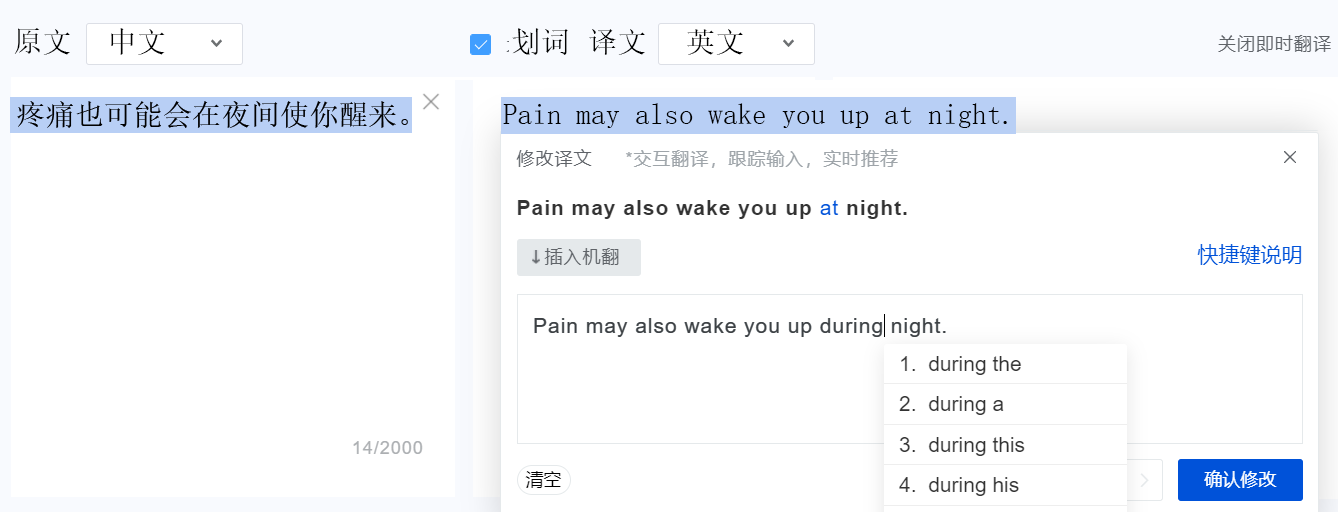
\includegraphics[scale=0.4]{./Chapter18/Figures/figure-transSmart.png}
%\setlength{\abovecaptionskip}{-0.2cm}
\caption{使用TranSmart系统进行交互式翻译的实例}
\label{fig:18-2}
\end{figure}
%----------------------------------------------

\parinterval 交互式机器翻译系统主要通过用户的反馈来提升译文的质量,不同类型的反馈信息则影响着系统最终的性能。根据反馈形式的不同,可以将交互式机器翻译分为以下几种:
\begin{itemize}
\vspace{0.5em}
\item 基于前缀的交互式机器翻译。早期的交互式机器翻译系统都是采用基于前缀的方式。基于翻译系统生成的初始译文,翻译人员从左到右检查翻译的正确性,并在第一个错误的位置进行更正。这为系统提供了一种双重信号:表明该位置上的单词必须是翻译人员修改过后的单词,并且该位置之前的单词都是正确的。之后系统根据已经检查过的前缀再生成后面的译文\upcite{DBLP:conf/acl/WuebkerGDHL16,Zens2003EfficientSF,DBLP:journals/coling/BarrachinaBCCCKLNTVV09,DBLP:journals/csl/PerisC19}。

\vspace{0.5em}
\item 基于片段的交互式机器翻译。根据用户提供的反馈来生成更好的翻译结果是交互式翻译系统的关键。而基于前缀的系统则存在一个严重的缺陷,当翻译系统获得确定的翻译前缀之后,再重新生成译文时会将原本正确的翻译后缀遗漏了,因此会引入新的错误。在基于片段的交互式机器翻译系统中,翻译人员除了纠正第一个错误的单词,还可以指定在未来迭代中保留的单词序列。之后系统根据这些反馈信号再生成新的译文\upcite{Peris2017InteractiveNM,DBLP:journals/mt/DomingoPC17}。

\vspace{0.5em}
\item 基于评分的交互式机器翻译。随着计算机算力的提升,有时会出现“机器等人”的现象,因此需要提升人参与交互的效率也是需要考虑的。与之前的系统不同,基于评分的交互式机器翻译系统不需要翻译人员选择、纠正或删除某个片段,而是使用翻译人员对译文的评分来强化机器翻译的学习\upcite{DBLP:journals/corr/abs-1805-01553,DBLP:conf/emnlp/NguyenDB17}。

\vspace{0.5em}
\end{itemize}

\parinterval 除此之外,基于在线学习的方法也受到了关注,这类方法也可以被看作是交互式翻译与增量训练的一种结合。用户总是希望翻译系统能从反馈中自动纠正以前的错误。当用户最终确认一个修改过后的译文后,翻译系统将源语言句子与该修正后的译文作为训练语料继续训练\upcite{DBLP:conf/acl/DomingoGEBHPCH19}。实际上,交互式机器翻译是机器翻译大规模应用的重要途径之一,它为打通翻译人员和机器翻译系统之间的障碍提供了手段。不过,交互式机器翻译也有许多挑战等待解决。一个是如何设计交互方式?理想的交互方式应该是更加贴近翻译人员输入文字的习惯,比如,利用输入法完成交互;另一个是如何把交互式翻译嵌入到翻译的生产流程里?这本身不完全是一个技术问题,可能需要更多的产品手段来求解。


%----------------------------------------------------------------------------------------
%    NEW SECTION
%----------------------------------------------------------------------------------------

\section{翻译结果的可干预性}

\parinterval 交互式机器翻译体现了一种用户的行为“干预”机器翻译结果的思想。实际上,在机器翻译出现错误时,人们总是希望用一种直接有效的方式“改变”译文,最短时间内达到改善翻译质量的目的。比如,如果机器翻译系统可以输出多个候选译文,用户可以在其中挑选最好的译文进行输出。也就是,人为干预了译文候选的排序过程。另一个例子是{\small\bfnew{翻译记忆}}\index{翻译记忆}(Translation Memory,TM\index{Translation Memory})。翻译记忆记录了高质量的源语言-目标语言句对,有时也可以被看作是一种先验知识或“记忆”。因此,当进行机器翻译时,使用翻译记忆指导翻译过程也可以被看作是一种干预手段\upcite{DBLP:conf/acl/WangZS13,DBLP:conf/aaai/XiaHLS19}。


\parinterval 虽然干预机器翻译系统的方式很多,最常用的还是对源语言特定片段翻译的干预,以期望最终句子的译文满足某些约束。这个问题也被称作{\small\bfnew{基于约束的翻译}}\index{基于约束的翻译} (Constraint-based Translation\index{Constraint-based Translation})。比如,在翻译网页时,需要保持译文中的网页标签与源文一致。另一个典型例子是术语翻译。在实际应用中,经常会遇到公司名称、品牌名称、产品名称等专有名词和行业术语,以及不同含义的缩写,比如,对于“小牛翻译”这个专有名词,不同的机器翻译系统给出的结果不一样:“Maverick translation”、“Calf translation”、“The mavericks translation”等等,而它正确的翻译应该为“NiuTrans”。 对于这些类似的特殊词汇,机器翻译引擎很难翻译得准确。一方面,因为模型大多是在通用数据集上训练出来的,并不能保证数据集能涵盖所有的语言现象。另一方面,即使是这些术语在训练数据中出现,它们通常也是低频的,模型不容易捕捉它们的规律。为了保证翻译的准确性,对术语翻译进行干预是十分有必要的,对领域适应等问题的求解也是非常有意义的。

\parinterval 就{\small\bfnew 词汇约束翻译}\index{词汇约束翻译}(Lexically Constrained Translation)\index{Lexically Constrained Translation}而言,在不干预的情况下让模型直接翻译出正确术语是很难的,因为术语的译文很可能是未登录词,因此必须人为提供额外的术语词典,那么我们的目标就是让模型的翻译输出遵守用户提供的术语约束。这个过程如图\ref{fig:18-3}所示。
%----------------------------------------------
\begin{figure}[htp]
\centering

%%% outline
%-------------------------------------------------------------------------
\begin{tikzpicture}[scale=0.8]
\tikzstyle{diction}=[align=center,rounded corners=2pt, draw,drop shadow,fill=green!20,font=\scriptsize]
\tikzstyle{word}=[align=center,anchor=west]
\begin{scope}

\node[word] (origin) at (0,0) {源文};
\node[word] (n1) at ([xshift=1em]origin.east){{\color{red} 小牛翻译}的总部在哪里?}; 

\node[word] (right) at ([yshift=-6em]origin.south west){译文};
\node[word] (n3) at ([xshift=1em]right.east){Where is the headquarters \\ of {\color{red} NiuTrans}?}; 

%\node[diction] (dic) at ([xshift=2em,yshift=-1.8em]n1.south east) {
%术语词典 \\
%小牛翻译 = NiuTrans \\
%......
%};
%\draw[->,red] ([yshift=-0.2em]dic.west)  .. controls +(west:2em) and +(south:2em) .. ( [xshift=-4em]n1.south) node[above,midway,font=\scriptsize]{};
\node[font=\scriptsize] at ([yshift=-2.3em,xshift=-6em]n1.south) {“小牛翻译”=“NiuTrans”};
\draw[->,very thick] ([yshift=-0.2em,xshift=-0.4em]n1.south) -- ([yshift=0.2em]n3.north);
%\draw[->,very thick] ([yshift=-0.2em,xshift=-0.2em]n2.south) -- ([yshift=0.2em]n3.north);

\end{scope}
\end{tikzpicture}






%\setlength{\abovecaptionskip}{-0.2cm}
\caption{词汇约束翻译过程}
\label{fig:18-3}
\end{figure}
%----------------------------------------------

\parinterval 在统计机器翻译中,翻译本质上是由短语和规则构成的推导,因此修改译文比较容易,比如,可以在一个源语言片段所对应的翻译候选集中添加希望得到的译文。而神经机器翻译是一个端到端模型,翻译过程本质上是连续空间中元素的一系列映射、组合和代数运算。虽然在模型训练阶段仍然可以通过修改损失函数等手段引入约束,但是在推断阶段进行直接干预并不容易,因为我们无法像修改符号系统那样直接修改模型(如短语翻译表)来影响译文生成。实践中主要有两种解决思路:

\begin{itemize}
\vspace{0.5em}
\item 强制生成。这种方法并不改变模型,而是在推断过程中按照一定的策略来实施约束,一般是修改束搜索算法以确保输出必须包含指定的词或者短语\upcite{DBLP:conf/acl/HokampL17,DBLP:conf/naacl/PostV18,DBLP:conf/wmt/ChatterjeeNTFSB17,DBLP:conf/naacl/HaslerGIB18},例如,在获得译文输出后,利用注意力机制获取词对齐,之后通过词对齐得到源语言和目标语言片段的对应关系,最后对指定译文片段进行强制替换。或者,对包含正确术语的翻译候选进行额外的加分,以确保推断时这样的翻译候选的排名足够靠前。

\vspace{0.5em}
\item 数据增强。这类方法通过修改机器翻译模型的训练数据来实现术语约束。通常根据术语词典对训练数据进行一定的修改,例如,将术语的译文添加到源文句子中,之后将原始语料库和合成语料库进行混合训练,期望模型能够学会自动利用术语信息来指导解码,或者是在训练数据中利用占位符来替换术语,待翻译完成后再进行还原\upcite{DBLP:conf/naacl/SongZYLWZ19,DBLP:conf/acl/DinuMFA19,DBLP:journals/corr/abs-1912-00567,DBLP:conf/ijcai/ChenCWL20}。

\vspace{0.5em}
\end{itemize}

\parinterval 强制生成的方法是在搜索策略上进行限制,与模型无关,这类方法能保证输出满足约束,但是会影响翻译速度。数据增强的方法是通过构造特定格式的数据让模型训练,从而让模型具有自动适应术语约束的能力,通常不会影响翻译速度,但并不能保证输出能满足约束。

\parinterval 此外,机器翻译在应用时通常还需要进行译前译后的处理,译前处理指的是在翻译前对源语言句子进行修改和规范,从而能生成比较通顺的译文,提高译文的可读性和准确率。在实际应用时,由于用户输入的形式多样,可能会包含比如术语、缩写、数学公式等,有些甚至可能还包含网页标签,因此对源文进行预处理是很有必要的。常见的处理工作包括格式转换、标点符号检査、术语编辑、标签识别等,待翻译完成后,则需要对机器译文进行进一步的编辑和修正,从而使其符合使用规范,比如进行标点、格式检查,术语、标签还原等,这些过程通常都是按照设定的处理策略自动完成的。另外,译文长度的控制、译文多样性的控制等也可以丰富机器翻译系统干预的手段(见{\chapterfourteen})。

%----------------------------------------------------------------------------------------
%    NEW SECTION
%----------------------------------------------------------------------------------------

\section{小设备机器翻译}

\parinterval 在机器翻译研究中,一般会假设计算资源是充足的。但是,在很多应用场景中,机器翻译使用的计算资源非常有限,比如,一些离线设备上没有GPU,而且CPU的处理能力也很弱,甚至内存也非常有限。这时,让模型变得更小、系统变得更快就成为了重要的需求。

\parinterval 本书中已经讨论了大量的可用于小设备上的机器翻译技术方法,例如:

\begin{itemize}
\vspace{0.5em}
\item 知识蒸馏({\chapterthirteen})。这种方法可以有效地将翻译能力从大模型迁移到小模型。

\vspace{0.5em}
\item 低精度存储及计算({\chapterfourteen})。可以使用量化的方式将模型压缩,同时整型计算也非常适合在CPU等设备上执行。

\vspace{0.5em}
\item 轻量模型结构({\chapterfourteen}和{\chapterfifteen})。对机器翻译模型的局部结构进行优化也是非常有效的手段,比如,使用更加轻量的卷积计算模块,或者使用深编码器-浅解码器等高效的结构。

\vspace{0.5em}
\item 面向设备的模型结构学习({\chapterfifteen})。可以把设备的存储及延时作为目标函数的一部分,自动搜索高效的翻译模型结构。

\vspace{0.5em}
\item 动态适应性模型\upcite{DBLP:conf/emnlp/WangXZ20,DBLP:journals/corr/BolukbasiWDS17,DBLP:conf/iclr/HuangCLWMW18}。模型可以动态调整大小或者计算规模,以达到在不同设备上平衡延时和精度的目的。比如,可以根据延时的要求,动态生成合适深度的神经网络进行翻译。

\vspace{0.5em}
\end{itemize}

\parinterval 此外,机器翻译系统的工程实现方式也是十分重要的,例如,编译器的选择、底层线性代数库的选择等等。有时候,使用与运行设备相匹配的编译器,会带来明显的性能提升\footnote{以神经机器翻译为例,张量计算部分大多使用C++等语言编写,因此编译器与设备的适配程度对程序的执行效率影响很大。}。如果希望追求更加极致的性能,甚至需要对一些热点模块进行修改。例如,在神经机器翻译中,矩阵乘法就是一个非常耗时的部分。但是这部分计算又与设备、矩阵的形状有很大关系。对于不同设备,根据不同的矩阵形状可以设计相应的矩阵乘法算法。不过,这部分工作对系统开发和硬件指令的使用水平要求较高。

\parinterval 另外,在很多系统中,机器翻译模块并不是单独执行,而是与其它的模块并发执行。这时,由于多个计算密集型任务存在竞争,处理器要进行更多的上下文切换,会造成程序变慢。比如,机器翻译和语音识别两个模块一起运行时{\footnote{在一些语音翻译场景中,由于采用了语音识别和翻译异步执行的方式,两个程序可能会并发。}},机器翻译的速度会有较明显的下降。对于这种情况,需要设计更好的调度机制。因此在一些同时具有CPU和GPU的设备上,可以考虑合理调度CPU和GPU的资源,增加两种设备可并行处理的内容,避免在某个处理器上的拥塞。

\parinterval 除了运行速度,模型过大也是限制其在小设备上运行的因素。在模型体积上,神经机器翻译模型具有天然的优势。因此,在对模型规模有苛刻要求的场景中,神经机器翻译是不二的选择。另外通过量化、剪枝、参数共享等方式,可以将模型大幅度压缩。

%----------------------------------------------------------------------------------------
%    NEW SECTION
%----------------------------------------------------------------------------------------

\section{机器翻译系统的部署}

\parinterval 除了在一些离线设备上使用机器翻译,更多时候机器翻译系统会部署在运算能力较强的服务器上。一方面随着神经机器翻译的大规模应用,在GPU服务器上部署机器翻译系统已经成为了常态。另一方面,GPU服务器的成本较高,而且很多应用中需要同时部署多个语言方向的系统。这时如何充分利用设备以满足大规模的翻译需求就成为了不可回避的问题。有几个方向值得尝试:

\begin{itemize}
\vspace{0.5em}
\item 对于多语言翻译的场景,使用多语言单模型翻译系统是一种很好的选择({\chaptersixteen})。当多个语种的数据量有限、使用频度不高时,这种方法可以很有效地解决翻译需求中的长尾部分。例如,一些线上机器翻译服务已经支持超过100种语言的翻译,其中大部分语言之间的翻译需求是相对低频的,因此使用同一个模型进行翻译可以大大节约部署和运维的成本。

\vspace{0.5em}
\item 使用基于枢轴语言的翻译也可以有效的解决多语言翻译问题({\chaptersixteen})。这种方法同时适合统计机器翻译和神经机器翻译,因此很早就使用在大规模机器翻译部署中。

\vspace{0.5em}
\item GPU部署中,由于GPU成本较高,因此可以考虑在单个GPU设备上部署多套不同的系统。如果这些系统之间的并发不频繁,翻译延时不会有明显增加。这种多个模型共享一个设备的方法比较适合翻译请求相对低频但是翻译任务又很多样的情况。

\vspace{0.5em}
\item 机器翻译大规模GPU部署对显存的使用也很严格。由于GPU显存较为有限,因此模型运行的显存消耗也是需要考虑的。一般来说,除了模型压缩和结构优化之外({\chapterfourteen}和{\chapterfifteen}),也需要对模型的显存分配和使用进行单独的优化。例如,使用显存池来缓解频繁申请和释放显存空间造成的延时。另外,也可以尽可能让同一个显存块保存生命期不重叠的数据,避免重复开辟新的存储空间。图\ref{fig:18-4}展示了一个显存复用的示例。

%----------------------------------------------
\begin{figure}[htp]
\centering
\begin{tabular}{c c}

\begin{tikzpicture}
\begin{scope}
% ,minimum height =1em,minimum width=2em
\tikzstyle{memory} = [draw,black,very thick,inner sep=2pt,rounded corners=0pt,fill=blue!20,minimum width=2em,minimum height=1.5em,anchor=west]
\tikzstyle{thread} = [very thick,inner sep=3.5pt,rounded corners=0pt,minimum width=3em,minimum height=1.5em]
\tikzstyle{word} = [inner sep=3.5pt,font=\scriptsize]

\node[thread] (one) at (0,0) {};
\node [word] at (one.north) {\scriptsize 数据1};
\draw[|-|,very thick] (-1.5em,0em) -- (1.6em,0em);

\node[thread,minimum width=5em] (two) at ([yshift=-1em,xshift=2.6em]one.south east) {};
\node [word] at (two.north) {\scriptsize 数据2};
\draw[|-|,very thick] (1.8em,-1.8em) -- (6.5em,-1.8em);

\node[thread,minimum width=4em] (three) at ([yshift=-1em,xshift=0.3em]two.south east) {};
\node [word] at (three.north) {\scriptsize 数据3};
\draw[|-|,very thick] (5em,-1.8*2em) -- (9em,-1.8*2em);

\node[thread,minimum width=2em] (four) at ([yshift=-1em,xshift=1.2em]three.south east) {};
\node [word] at (four.north) {\scriptsize 数据4};
\draw[|-|,very thick] (9.3em,-1.8*3em) -- (11em,-1.8*3em);

\node [memory] (mone) at ([yshift=4em,xshift=1em]one.north) {};
\node [memory] (mtwo) at ([xshift=0em]mone.east) {};
\node [memory] (mthree) at ([xshift=0em]mtwo.east) {};
\node [memory] (mfour) at ([xshift=0em]mthree.east) {};

\draw[->,very thick] (-0.8,-2.5) -- (4.7,-2.5);
\draw[->,very thick] (-0.8,-2.5) -- (-0.8,1);
 
\node [word] (time) at ([yshift=-1.5em,xshift=0.3em]four.south) {\scriptsize 时间线};
\node [word] (time) at ([yshift=1.5em,xshift=-2.2em]one.west) {\scriptsize 数据};

\draw [->,dashed,line width=0.7pt] ([yshift=0.5em]one.north) .. controls +(north:1.5em) and +(south:1.5em) .. ([yshift=-0.2em]mone.south);
\draw [->,dashed,line width=0.7pt] ([yshift=0.5em]two.north) -- ([yshift=-0.2em]mtwo.south);
\draw [->,dashed,line width=0.7pt] ([yshift=0.5em,xshift=0.5em]three.north) .. controls +(north:3.5em) and +(south:4.5em) .. ([yshift=-0.2em]mthree.south);
\draw [->,dashed,line width=0.7pt] ([yshift=0.5em]four.north) .. controls +(north:4.5em) and +(south:4.5em) .. ([yshift=-0.2em]mfour.south);

\node [word] at ([yshift=-6em]two.south) {(a) 显存不复用};

%占位
\node[word] at ([xshift=1em]four.east) {};

\node [word] at ([xshift=1.5em,yshift=5.6em]one.north) {\scriptsize 显存};

\begin{pgfonlayer}{background}
\node [rectangle,inner sep=0.5em,rounded corners=1pt,minimum width=10em,minimum height=3.6em,fill=gray!10,drop shadow] at ([yshift=6.6em,xshift=1em]two.north) {};
\end{pgfonlayer}

\end{scope}
\end{tikzpicture}
&
\begin{tikzpicture}
\begin{scope}
%\tikzstyle{memory} = [draw,black,very thick,inner sep=2pt,rounded corners=0pt,fill=blue!20,minimum width=2em,minimum height=1.5em,anchor=west]
%\tikzstyle{thread} = [draw,black,very thick,inner sep=3.5pt,rounded corners=0pt,fill=green!20,minimum width=3em,minimum height=1.5em]
\tikzstyle{memory} = [draw,black,very thick,inner sep=2pt,rounded corners=0pt,fill=blue!20,minimum width=2em,minimum height=1.5em,anchor=west]
\tikzstyle{thread} = [very thick,inner sep=3.5pt,rounded corners=0pt,minimum width=3em,minimum height=1.5em]
\tikzstyle{word} = [inner sep=3.5pt,font=\scriptsize]

\node[thread] (one) at (0,0) {};
\node [word] at (one.north) {\scriptsize 数据1};
\draw[|-|,very thick] (-1.5em,0em) -- (1.6em,0em);

\node[thread,minimum width=5em] (two) at ([yshift=-1em,xshift=2.6em]one.south east) {};
\node [word] at (two.north) {\scriptsize 数据2};
\draw[|-|,very thick] (1.8em,-1.8em) -- (6.5em,-1.8em);

\node[thread,minimum width=4em] (three) at ([yshift=-1em,xshift=0.3em]two.south east) {};
\node [word] at (three.north) {\scriptsize 数据3};
\draw[|-|,very thick] (5em,-1.8*2em) -- (9em,-1.8*2em);

\node[thread,minimum width=2em] (four) at ([yshift=-1em,xshift=1.2em]three.south east) {};
\node [word] at (four.north) {\scriptsize 数据4};
\draw[|-|,very thick] (9.3em,-1.8*3em) -- (11em,-1.8*3em);

\node [memory] (mone) at ([yshift=4em,xshift=1em]one.north) {};
\node [memory] (mtwo) at ([xshift=0em]mone.east) {};
\node [memory,fill=white,minimum width=4em] (mthree) at ([xshift=0em]mtwo.east) {};
%\node [memory,fill=white] (mfour) at ([xshift=0em]mthree.east) {};

\draw[->,very thick] (-0.8,-2.5) -- (4.7,-2.5);
\draw[->,very thick] (-0.8,-2.5) -- (-0.8,1);

\node [word] (time) at ([yshift=-1.5em,xshift=0.3em]four.south) {\scriptsize 时间线};
\node [word] (time) at ([yshift=1.5em,xshift=-2.2em]one.west) {\scriptsize 数据};

\draw [->,dashed,line width=0.7pt] ([yshift=0.5em]one.north) .. controls +(north:1.5em) and +(south:1.5em) .. ([yshift=-0.2em,xshift=-0.4em]mone.south);
\draw [->,dashed,line width=0.7pt] ([yshift=0.5em]two.north) .. controls +(north:3.5em) and +(south:3.5em) .. ([yshift=-0.2em,xshift=0.4em]mone.south);
\draw [->,dashed,line width=0.7pt] ([yshift=0.5em,xshift=0.5em]three.north) .. controls +(north:3.5em) and +(south:3.5em) .. ([yshift=-0.2em,xshift=-0.4em]mtwo.south);
\draw [->,dashed,line width=0.7pt] ([yshift=0.5em]four.north) .. controls +(north:4.5em) and +(south:3.5em) .. ([yshift=-0.2em,xshift=0.4em]mtwo.south);

\node [word] at ([xshift=1.5em,yshift=5.6em]one.north) {\scriptsize 显存};

\node [word] at ([yshift=-6em]two.south) {(b) 显存复用};

\begin{pgfonlayer}{background}
\node [rectangle,inner sep=0.5em,rounded corners=1pt,minimum width=10em,minimum height=3.6em,fill=gray!10,drop shadow] at ([yshift=6.6em,xshift=1em]two.north) {};
\end{pgfonlayer}


\end{scope}
\end{tikzpicture}

\end{tabular}
%\setlength{\abovecaptionskip}{-0.2cm}
\caption{显存不复用与显存复用的示例}
\label{fig:18-4}
\end{figure}
%----------------------------------------------
\vspace{0.5em}
\item 在翻译请求高并发的场景中,使用批量翻译也是有效利用GPU设备的方式。不过,机器翻译是一个处理不定长序列的任务,输入的句子长度差异较大。而且,由于译文长度无法预知,进一步增加了不同长度的句子所消耗计算资源的不确定性。这时,可以让长度相近的句子在一个批次里处理,减小由于句子长度不统一造成的补全过多、设备利用率低的问题。例如,可以按输入句子长度范围分组。 也可以设计更加细致的方法对句子进行分组,以最大化批量翻译中设备的利用率\upcite{DBLP:journals/corr/abs-2010-05680}。

\vspace{0.5em}
\end{itemize}

\parinterval 除了上述问题,如何对多设备环境下进行负载均衡、容灾处理等都是大规模机器翻译系统部署中需要考虑的。有时候,甚至统计机器翻译系统也可以与神经机器翻译系统混合使用。由于统计机器翻译系统对GPU资源的要求较低,纯CPU部署的方案也相对成熟。因此,可以作为GPU机器翻译服务的灾备。此外,在有些任务,特别是某些低资源翻译任务上,统计机器翻译仍然具有优势。

%----------------------------------------------------------------------------------------
%    NEW SECTION
%----------------------------------------------------------------------------------------

\section{机器翻译的应用场景}

\parinterval 机器翻译有着十分广泛的应用,这里列举了一些常见的应用场景:
\begin{itemize} 
\item {\small\bfnew{网页翻译}}。进入信息爆炸的时代之后,互联网上海量的数据随处可得,然而由于不同国家和地区语言的差异,网络上的数据也呈现出多语言的特性。当人们在遇到包含不熟悉语言的网页时,无法及时有效地获取其中的信息。因此,对不同语言的网页进行翻译是必不可少的一步。由于网络上的网页数不胜数,依靠人工对网页进行翻译是不切实际的,相反,机器翻译十分适合这个任务。目前,市场上有很多浏览器提供网页翻译的服务,极大地降低了人们从网络上获取不同语言信息的难度。

\item {\small\bfnew{科技文献翻译}}。在专利等科技文献翻译中,往往需要将文献翻译为英语或者其他语言,比如摘要翻译。以往这种翻译工作通常由人工来完成。由于对翻译结果的质量要求较高,因此要求翻译人员具有相关专业的背景知识,这导致翻译人员资源稀缺。特别是,近几年国内专利申请数不断增加,这给人工翻译带来了很大的负担。相比于人工翻译,机器翻译可以在短时间内完成大量的专利翻译,同时结合术语词典和人工校对等方式,可以保证专利的翻译质量。另外,以专利为代表的科技文献往往具有很强的领域性,针对各类领域文本进行单独优化,机器翻译的品质可以大大提高。因此,机器翻译在专利翻译等行业有十分广泛的应用前景。

\item {\small\bfnew{视频字幕翻译}}。随着互联网的普及,人们可以通过互联网接触到大量境外影视作品。由于人们可能没有相应的外语能力,通常需要翻译人员对字幕进行翻译。因此,这些境外视频的传播受限于字幕翻译的速度和准确度。现在的一些视频网站在使用语音识别为视频生成源语言字幕的同时,通过机器翻译技术为各种语言的受众提供质量尚可的目标语言字幕,这种方式为人们提供了极大的便利。

\item {\small\bfnew{社交}}。社交是人们的重要社会活动。人们可以通过各种各样的社交软件做到即时通讯,进行协作或者分享自己的观点。然而受限于语言问题,人们的社交范围往往不会超出自己所掌握的语种范围,很难方便地进行跨语言社交。随着机器翻译技术的发展,越来越多的社交软件开始支持自动翻译,用户可以轻易地将各种语言的内容翻译成自己的母语,方便了人们的交流,让语言问题不再成为社交的障碍。

\item {\small\bfnew{同声传译}}。在一些国际会议中,与会者来自许多不同的国家,为了保证会议的流畅,通常需要专业翻译人员进行同声传译。同声传译需要在不打断演讲的同时,不间断地将讲话内容进行口译,对翻译人员的要求极高。现在,一些会议开始采用语音识别来将语音转换成文本,同时使用机器翻译技术进行翻译的方式,达到同步翻译的目的。这项技术已经得到了多个企业的关注,并在很多重要会议上进行尝试,取得了很好的反响。不过同声传译达到可以真正使用的程度还需一定时间的打磨,特别是会议场景下,准确进行语音识别和翻译仍然具有挑战性。

\item {\small\bfnew{中国传统语言文化的翻译}}。中国几千年的历史留下了极为宝贵的文化遗产,而其中,文言文作为古代书面语,具有言文分离、行文简练的特点,易于流传。言文分离的特点使得文言文和现在的标准汉语具有一定的区别。为了更好发扬中国传统文化,需要对文言文进行翻译。而文言文古奥难懂,人们需要具备一定的文言文知识背景才能准确翻译。机器翻译技术也可以帮助人们快速完成文言文的翻译。除此之外,机器翻译技术同样可以用于古诗生成和对联生成等任务。

\item {\small\bfnew{全球化}}。在经济全球化的今天,很多企业都有国际化的需求,企业员工或多或少地会遇到一些跨语言阅读和交流的情况,比如阅读进口产品的说明书,跨国公司之间的邮件、说明文件等等。相比于成本较高的人工翻译,机器翻译往往是一种很好的选择。在一些质量要求不高的翻译场景中,机器翻译可以得到应用。

\item {\small\bfnew{翻译机/翻译笔}}。出于商务、学术交流或者旅游的目的,人们在出国时会面临着跨语言交流的问题。近几年,随着出境人数的增加,不少企业推出了翻译机产品。通过结合机器翻译、语音识别和图像识别技术,翻译机实现了图像翻译和语音翻译的功能。用户可以很便捷地获取一些外语图像文字和语音信息,同时可以通过翻译机进行对话,降低跨语言交流门槛。类似地,翻译笔等应用产品可以通过划词翻译的方式,对打印材料中的外语文字进行翻译。

\item {\small\bfnew{译后编辑}}。翻译结果后编辑是指在机器翻译的结果之上,通过少量的人工编辑来进一步完善机器译文。在传统的人工翻译过程中,翻译人员完全依靠人工的方式进行翻译,这虽然保证了翻译质量,但是时间成本高。相对应地,机器翻译具有速度快和成本低的优势。在一些领域,目前的机器翻译质量已经可以很大程度上减少翻译人员的工作量,翻译人员可以在机器翻译的辅助下,花费相对较小的代价来完成翻译。

\end{itemize}

%----------------------------------------------------------------------------------------
%    NEW SECTION
%----------------------------------------------------------------------------------------

%\section{拓展思考}
